% Options for packages loaded elsewhere
\PassOptionsToPackage{unicode}{hyperref}
\PassOptionsToPackage{hyphens}{url}
\PassOptionsToPackage{dvipsnames,svgnames,x11names}{xcolor}
%
\documentclass[
  12pt,
]{article}
\usepackage{amsmath,amssymb}
\usepackage{iftex}
\ifPDFTeX
  \usepackage[T1]{fontenc}
  \usepackage[utf8]{inputenc}
  \usepackage{textcomp} % provide euro and other symbols
\else % if luatex or xetex
  \usepackage{unicode-math} % this also loads fontspec
  \defaultfontfeatures{Scale=MatchLowercase}
  \defaultfontfeatures[\rmfamily]{Ligatures=TeX,Scale=1}
\fi
\usepackage{lmodern}
\ifPDFTeX\else
  % xetex/luatex font selection
\fi
% Use upquote if available, for straight quotes in verbatim environments
\IfFileExists{upquote.sty}{\usepackage{upquote}}{}
\IfFileExists{microtype.sty}{% use microtype if available
  \usepackage[]{microtype}
  \UseMicrotypeSet[protrusion]{basicmath} % disable protrusion for tt fonts
}{}
\makeatletter
\@ifundefined{KOMAClassName}{% if non-KOMA class
  \IfFileExists{parskip.sty}{%
    \usepackage{parskip}
  }{% else
    \setlength{\parindent}{0pt}
    \setlength{\parskip}{6pt plus 2pt minus 1pt}}
}{% if KOMA class
  \KOMAoptions{parskip=half}}
\makeatother
\usepackage{xcolor}
\usepackage[margin=1in]{geometry}
\usepackage{longtable,booktabs,array}
\usepackage{calc} % for calculating minipage widths
% Correct order of tables after \paragraph or \subparagraph
\usepackage{etoolbox}
\makeatletter
\patchcmd\longtable{\par}{\if@noskipsec\mbox{}\fi\par}{}{}
\makeatother
% Allow footnotes in longtable head/foot
\IfFileExists{footnotehyper.sty}{\usepackage{footnotehyper}}{\usepackage{footnote}}
\makesavenoteenv{longtable}
\usepackage{graphicx}
\makeatletter
\def\maxwidth{\ifdim\Gin@nat@width>\linewidth\linewidth\else\Gin@nat@width\fi}
\def\maxheight{\ifdim\Gin@nat@height>\textheight\textheight\else\Gin@nat@height\fi}
\makeatother
% Scale images if necessary, so that they will not overflow the page
% margins by default, and it is still possible to overwrite the defaults
% using explicit options in \includegraphics[width, height, ...]{}
\setkeys{Gin}{width=\maxwidth,height=\maxheight,keepaspectratio}
% Set default figure placement to htbp
\makeatletter
\def\fps@figure{htbp}
\makeatother
\setlength{\emergencystretch}{3em} % prevent overfull lines
\providecommand{\tightlist}{%
  \setlength{\itemsep}{0pt}\setlength{\parskip}{0pt}}
\setcounter{secnumdepth}{5}
\usepackage{setspace} \usepackage{amssymb} \usepackage{amsmath} \setstretch{1.15} \usepackage{float} \floatplacement{figure}{t}
\ifLuaTeX
  \usepackage{selnolig}  % disable illegal ligatures
\fi
\IfFileExists{bookmark.sty}{\usepackage{bookmark}}{\usepackage{hyperref}}
\IfFileExists{xurl.sty}{\usepackage{xurl}}{} % add URL line breaks if available
\urlstyle{same}
\hypersetup{
  colorlinks=true,
  linkcolor={cyan},
  filecolor={Maroon},
  citecolor={Blue},
  urlcolor={cyan},
  pdfcreator={LaTeX via pandoc}}

\title{~\Large A Comparison of Batter Performance and League Quality
Across Domestic T-20 Cricket Leagues}
\author{\large Matthew Stuart\(^{1,2}\), Hassan Raffique\(^{3}\), Leigha
DeRango\(^{1,2}\)\\
\large Gregory J. Matthews\(^{1,2}\)\\
\vspace{-1.1mm}\\
\large \(^1\) Department of Mathematics and Statistics, Loyola
University Chicago, Chicago, IL, USA \vspace{-1.1mm}\\
\large \(^2\) Center for Data Science and Consulting, Loyola University
Chicago, Chicago, IL, USA \vspace{-1.1mm}\\
\large \(^3\) Syracuse University, Syracuse, NY, USA \vspace{-1.1mm}\\
\large \(^+\) Corresponding:
\href{mailto:mstuart1@luc.edu}{\nolinkurl{mstuart1@luc.edu}}
\vspace{-1.1mm}}
\date{}

\begin{document}
\maketitle
\begin{abstract}
Wicked Googly \vspace{2mm}\\
\emph{Keywords}: Cricket
\end{abstract}

\newcommand{\iid}{\overset{iid}{\sim}}

Abstract:

This paper investigates batter performance across major domestic
Twenty20 (T20) cricket leagues to understand how player effectiveness
varies by competition context. Using a comprehensive dataset comprising
individual match-level batting records from the Indian Premier League
(IPL), Big Bash League (BBL), Caribbean Premier League (CPL), Pakistani
Super League (PSL), and South Africa 20 (SAT), we fit a multinomial
regression model for the number of runs scored per bowled ball
accounting for batter and league conditions as well as in-match effects.
A hierarchical modeling framework utilizing a Bayesian framework is
employed to quantify both player-specific ability and league-specific
correlations, allowing for quantifiable player comparisons across
leagues and the estimation of league-adjusted performance ratings. Our
findings will offer insights into talent evaluation and the
transferability of performance across T20 competitions.

\newpage

\hypertarget{sec:intro}{%
\section{Introduction}\label{sec:intro}}

openWAR and cricWAR.

In the game of cricket, the number of runs scored on a particular pitch
typically ranges between 0 and 6 (though theoretically values larger
than 6 are possible, they are rare and do not occur at all in our
particular data set).

\hypertarget{sec:data}{%
\section{Data}\label{sec:data}}

\begin{longtable}[]{@{}rrrrrr@{}}
\toprule\noalign{}
year & BBL & CPL & IPL & PSL & SAT \\
\midrule\noalign{}
\endhead
\bottomrule\noalign{}
\endlastfoot
2015 & 8 & 6 & 8 & 5 & NA \\
2016 & 8 & 6 & 8 & 5 & NA \\
2017 & 8 & 6 & 8 & 6 & NA \\
2018 & 8 & 6 & 8 & 6 & NA \\
2019 & 8 & 6 & 8 & 6 & NA \\
2020 & 8 & 6 & 8 & 6 & NA \\
2021 & 8 & 6 & 8 & 6 & NA \\
2022 & 8 & 6 & 10 & 6 & 6 \\
2023 & 8 & 6 & 10 & 6 & 6 \\
2024 & NA & 6 & 10 & NA & NA \\
\end{longtable}

We have data from the Indian Premier League (IPL), Big Bash League
(BBL), Caribbean Premier League (CPL), Pakistani Super League (PSL), and
South Africa 20 (SAT), consisting of 408056 balls thrown, providing
\(L = 5\) leagues worth of data. From 2015 - 2021, the IPL, the longest
running T20 league, had 8 teams followed by 10 teams in the 2022 season.
In addition, the SAT was first contested in the 2022-2023 season.

\begin{longtable}[]{@{}rrrrrr@{}}
\toprule\noalign{}
year & BBL & CPL & IPL & PSL & SAT \\
\midrule\noalign{}
\endhead
\bottomrule\noalign{}
\endlastfoot
2015 & 7586 & 7268 & 13641 & 5413 & NA \\
2016 & 8259 & 6785 & 14096 & 5418 & NA \\
2017 & 10263 & 7708 & 13849 & 7728 & NA \\
2018 & 13576 & 7890 & 14286 & 8077 & NA \\
2019 & 13503 & 8064 & 14293 & 6144 & NA \\
2020 & 14125 & 7308 & 14510 & 4289 & NA \\
2021 & 14234 & 8042 & 14413 & 12978 & NA \\
2022 & 14168 & 7349 & 17912 & 8209 & 7392 \\
2023 & 9277 & 7233 & 17863 & 7806 & 7400 \\
2024 & NA & 2598 & 17103 & NA & NA \\
\end{longtable}

Runs in cricket are either scored by running back and forth between the
wickets once the ball is put into play (generally resulting in 1 or 2
runs, but theoretically any value is possible). In addition, a ball that
is hit in the air over the boundary (termed a ``boundary'') is worth 6
runs and if the ball rolls to the boundary or bounces in the field of
play and then clears the boundary this is worth 4 runs (termed a
``boundary 4''). As a result the distribution of runs scored on a a
particular pitch has large peaks are 0 and 1 with a big drop off from 1
to 2. Values of 3 and 5 are extremely rare accounting for only 0.38\%
and 0.02\% of values across all pitches in our data set. Values of 4 and
6 spike because of boundaries and boundary fours and together account
for 16.16\% of all values.

\begin{figure}

{\centering 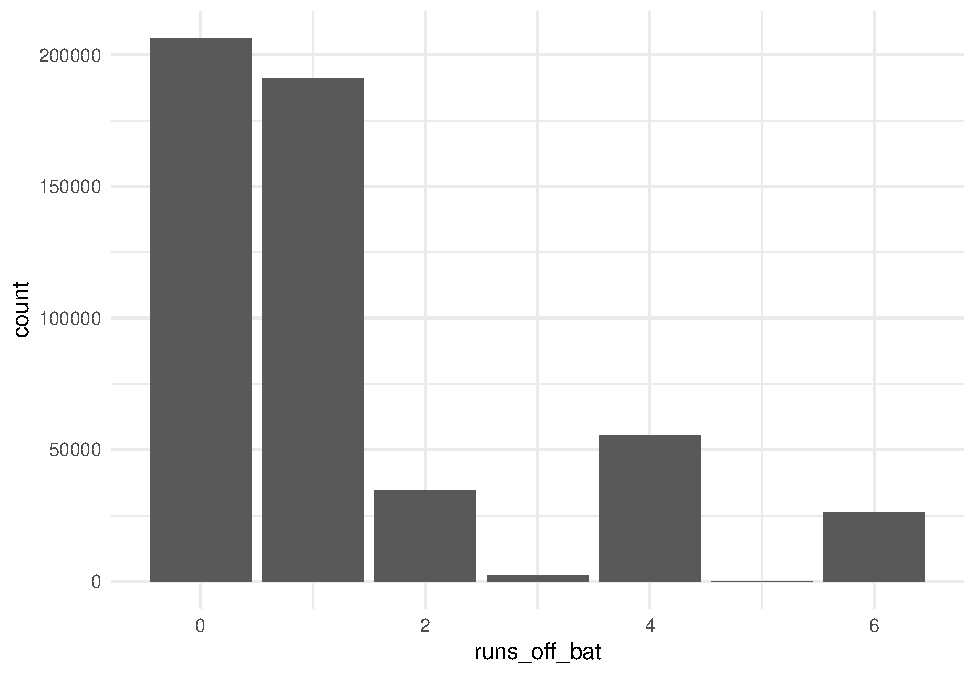
\includegraphics{paper_files/figure-latex/bar-1} 

}

\caption{Bar Plot of the number of runs scored of a particular ball}\label{fig:bar}
\end{figure}

\hypertarget{sec:models}{%
\section{Models}\label{sec:models}}

Figure \ref{fig:bar} displays a histogram of the number of runs scored
per ball in IPL, BBL, CPL, PSL, and SAT matches from 2015-2024,
consisting of \(n = 408,056\) balls thrown. It is likely that a
distribution used for modelling counts, such as the Poisson
distribution, will violate the necessary assumptions. For this reason,
we treat this as a classification problem and fit the number of runs
scored per ball, \(Y_i\), by a multinomial distribution. In addition, we
exclude any balls that scored three or five runs because of their
prementioned rarity of occuring. Thus, we are left with a dataset
consisting of \(n = 406,454\) balls thrown.

We utilize a mixed effects model, incorporating fixed effects for the
general in-match situations as well as random effects for the
variability of the bowler, batter, and runner. Denote \(Y_i\) as the
number of runs scored on ball \(i = 1,\dots,n\) and \(\boldsymbol{X}_i\)
as the vector of covariates for the fixed effects of ball \(i\). Table
@ref(tab:covariates) provides a description of the covariates for the
fixed effects of our model. The model is specified with four logit
transformations relative to the event \(Y_i = 0\), or, written
explicitly \begin{equation}
\log\left(\frac{P(Y_i = k | \boldsymbol{X}_i)}{P(Y_i = 0 | \boldsymbol{X}_i)}\right) = \boldsymbol{X}_i \boldsymbol{\beta}_k + u_{k, b_it_i} + s_{k,v_i} \label{model}
\end{equation} for \(k \in \{1,2,4,6\}\) where \(\boldsymbol{\beta}_k\)
is the fixed effect for scoring \(k\) runs, \(u_{k,b_it_i}\), is the
random effect for the batter(\(b_i\)) and year(\(t_i\)), and
\(s_{k,v_i}\) is the random effect for venue for ball \(i\),
respectively. For the batter random effects \({u}_{k,bt}\), we model the
random effects for each \(b\) via an AR1 process. More specifically, for
each \(k \in \{1,2,4,6\}\), we set \begin{align}
{u}_{k,bt} & \sim \mathcal{N}(\rho_k {u}_{k,b(t-1)},\sigma_{k}), \nonumber \\ 
{u}_{k,b1} & \sim \mathcal{N}(0,\frac{\sigma_{k}}{1-\rho_k^2})\label{ranefs_bat}
\end{align}

for \(t = 2,\cdots,T\). For the random effects for venue, we assume
\begin{align}
{s}_{k,v} & \sim \mathcal{N}(0,\tau_{k}), \label{ranefs_ven}
\end{align}

Given the size of the random effects, the size of our free, unknown
parameter vector
\(\boldsymbol{\Theta} = \{\boldsymbol{\beta}_k,\boldsymbol{u}_k, \boldsymbol{v}_k,\tau_k,\sigma_k: k \in \{1,2,4,6\}\}\)
is 43,740. To handle such a large parameter vector as well as the
complicated structure of our model, we perform a Bayesian analysis on
the data with prior distributions and sampling procedure outlined in the
supplemental file.

\begin{longtable}[]{@{}
  >{\raggedright\arraybackslash}p{(\columnwidth - 2\tabcolsep) * \real{0.1975}}
  >{\raggedright\arraybackslash}p{(\columnwidth - 2\tabcolsep) * \real{0.8025}}@{}}
\caption{Description of covariates for fixed effects of
model}\tabularnewline
\toprule\noalign{}
\begin{minipage}[b]{\linewidth}\raggedright
Variable
\end{minipage} & \begin{minipage}[b]{\linewidth}\raggedright
Variable.Description
\end{minipage} \\
\midrule\noalign{}
\endfirsthead
\toprule\noalign{}
\begin{minipage}[b]{\linewidth}\raggedright
Variable
\end{minipage} & \begin{minipage}[b]{\linewidth}\raggedright
Variable.Description
\end{minipage} \\
\midrule\noalign{}
\endhead
\bottomrule\noalign{}
\endlastfoot
First Innings & Indicator for the 1st innings of the match \\
Balls Remaining & Number of balls remaining in the innings \\
Runs to Win & Number of runs remaining to score to win the match (2nd
innings) \\
Runs Scored & Number of runs scored in the innings up to current ball \\
Wickets Lost & Number of wickets lost in the innings up to current
ball \\
League & League in which the match is played \\
\end{longtable}

\hypertarget{sec:results}{%
\section{Results}\label{sec:results}}

\hypertarget{sec:conclusions}{%
\section{Discussion, Future work and
conclusions}\label{sec:conclusions}}

\hypertarget{acknowledgements}{%
\section*{Acknowledgements}\label{acknowledgements}}
\addcontentsline{toc}{section}{Acknowledgements}

\hypertarget{supplementary-material}{%
\section*{Supplementary Material}\label{supplementary-material}}
\addcontentsline{toc}{section}{Supplementary Material}

All code for reproducing the analyses in this paper is publicly
available at \url{https://github.com/gjm112/cricketIPL}

\hypertarget{bayesian-priors-and-posterior-sampling}{%
\subsection{Bayesian priors and posterior
sampling}\label{bayesian-priors-and-posterior-sampling}}

In the data analysis outlined in Section \ref{sec:models} of the main
manuscript, we set the following prior distributions: \begin{align}
  \beta_{p,k} & \overset{iid}{\sim}\mathcal{N}(0,5),\nonumber\\
  \sigma_{k} & \overset{iid}{\sim}\mathcal{N}(0,1)I(\sigma_{k} > 0),\nonumber\\
  \tau_{k} & \overset{iid}{\sim}\mathcal{N}(0,1)I(\tau_{k} > 0),\nonumber\\
  \rho_{k} & \overset{iid}{\sim}\mathcal{N}(1,1)I(-1 < \rho_{k} < 1),
\end{align} for \(p = 1,\dots,10\) and \(k \in \{1,2,4,6\}\). We used
STAN to obtain 4000 posterior draws from our parameter set
\(\boldsymbol{\Theta} = \{\boldsymbol{\beta}_k,\boldsymbol{u}_k, \boldsymbol{v}_k,\tau_k,\sigma_k: k \in \{1,2,4,6\}\}\)

\hypertarget{references}{%
\section{References}\label{references}}

\end{document}
